\documentclass[11pt]{article}

% ---------- Page & typography ----------
\usepackage[margin=1in]{geometry}
\usepackage[T1]{fontenc}
\usepackage[utf8]{inputenc}
\usepackage[english]{babel}
\usepackage{lmodern}
\usepackage{microtype}
\usepackage{float}
\usepackage{graphicx}
\usepackage{setspace}
\usepackage{threeparttable}
\usepackage[italicdiff]{physics}
\usepackage{tikz, pgfplots, pgfplotstable}
\usepackage{algorithm}
\usepackage{algpseudocode}
\usepackage{booktabs}
\usepackage{multirow}
\usepackage{tabularx}
\usepackage{array}
\usepackage{hyperref}
\usepackage[table]{xcolor}
\usepackage{multicol}
\usepackage{enumitem}
\usepackage{mdframed}
\usepackage{siunitx}
\usepackage{adjustbox}
\usepackage{longtable}
\usepackage{pgfmath}
\usepackage{collcell}
\usepackage{caption}
\usepackage{subcaption}
\usepackage{fontawesome5}
\usepackage{listings}
\usepackage{siunitx}
\usepackage{numprint}

\usepackage{xcolor}

\lstset{
    basicstyle=\ttfamily\small,
    keywordstyle=\color{blue},
    stringstyle=\color{orange},
    commentstyle=\color{gray}\itshape,
    showstringspaces=false,
    breaklines=true,
    frame=single,
    language=Python
}


\DeclareUnicodeCharacter{2061}{}

\usetikzlibrary{positioning, arrows, arrows.meta, shapes, shapes.geometric,
                decorations, decorations.pathmorphing, decorations.text,
                fit, calc, backgrounds}

\usepgfplotslibrary{patchplots, colormaps}

% ---------- Colours ----------
\definecolor{ForestGreen}{RGB}{34,139,34}
\definecolor{PolyBlue}{RGB}{30,80,162}
\definecolor{PolyGold}{RGB}{200,160,0}
\definecolor{LightGray}{RGB}{245,245,245}

% ---------- Siunitx ----------
\sisetup{detect-all, table-number-alignment=center,
         round-mode=places, round-precision=3}

% ---------- P&L gradient cells ----------
\newcommand{\pnlcell}[1]{%
  \begingroup
  \ifdim #1pt < -20pt \cellcolor{red!40}#1%
  \else\ifdim #1pt < 0pt \cellcolor{red!15}#1%
  \else\ifdim #1pt < 20pt \cellcolor{green!15}#1%
  \else \cellcolor{green!40}#1%
  \fi\fi\fi
  \endgroup
}

% ---------- Hyperref ----------
\hypersetup{colorlinks=true, linkcolor=PolyBlue,
            citecolor=black, urlcolor=PolyBlue}
\onehalfspacing

% ---------- Maths ----------
\usepackage{amsmath, amssymb, amsthm, mathtools}
\makeatletter
\@removefromreset{equation}{section}
\makeatother
\renewcommand{\theequation}{\arabic{equation}}

% ---------- Lists ----------
\setlist{itemsep=2pt, topsep=4pt}
\setlength{\parindent}{0pt}
\renewcommand{\arraystretch}{1.2}

% ---------- Column types ----------
\newcolumntype{L}{>{\raggedright\arraybackslash}X}
\newcolumntype{C}{>{\centering\arraybackslash}m{0.22\linewidth}}
\newcolumntype{R}{>{\raggedleft\arraybackslash}X}

% ---------- Section input helper ----------
% \inputsection{filename} — pulls from sections/
\newcommand{\inputsection}[1]{\input{sections/#1}}




% ==========================================================
%  TITLE
% ==========================================================
\title{\vspace{0.2em}\textbf{FIN42110 - Financial Data Science\\[1.2em]
Detecting Informed Trading on Polymarket:\\[0.5em]
A Geopolitical Prediction Market Analysis}}
\date{April 2026}

\begin{document}
\maketitle

\begin{center}

\includegraphics[width=0.45\textwidth]{figures/smurfit_colour_transparent.png}

\includegraphics[width=0.45\textwidth]{figures/polymarket_logo.png}

\vspace{1.2em}
{\large \faGithub\;
\href{https://github.com/johnstew324/polymarket-whale-watch}{%
\texttt{johnstew324/polymarket-whale-watch}}}
\end{center}

\newpage
% ---------- Details table ----------
\begin{tabularx}{\textwidth}{>{\bfseries}l L >{\bfseries}l L}
\toprule
Student Name 1 & Oisín Moffatt  & Student Number 1 & 21510573 \\
Student Name 2 & John Stewart   & Student Number 2 & 25210841 \\
Student Name 3 & Adam Ajmal     & Student Number 3 & 20309543 \\
Module Title   & Financial Data Science for Trading \& Risk Management
               & Module Co-ordinator & Dr Richard McGee \\
\bottomrule
\end{tabularx}

\vspace{1.2cm}

{\bfseries Procedures for Submission and Late Submission:} ensure that you
have checked the School's procedures for the submission of assessments.
Note: There are penalties for the late submission of assessments. For
further information please see the University's Policy on Late Submission
of Coursework,
\href{http://www.ucd.ie/registrar/}{http://www.ucd.ie/registrar/}.

\vspace{0.7cm}

{\bfseries Plagiarism:} the unacknowledged inclusion of another person's
writings or ideas or works, in any formally presented work (including
essays, examinations, projects, laboratory reports or presentations). The
penalties associated with plagiarism are designed to impose sanctions that
reflect the seriousness of the University's commitment to academic
integrity. Ensure that you have read the University's Briefing for Students
on Academic Integrity and Plagiarism and the UCD Plagiarism Statement,
Plagiarism Policy and Procedures,
\href{http://www.ucd.ie/registrar/}{http://www.ucd.ie/registrar/}.

\vspace{1.0cm}

\begin{mdframed}[linewidth=0.6pt]
{\bfseries Declaration of Authorship}

We declare that all material in this assessment is our own work except
where there is clear \underline{acknowledgement} and appropriate reference
to the work of others.

\vspace{0.6cm}
Signed\dotfill\ Oisín Moffatt\dotfill\par
\vspace{0.2cm}
Signed\dotfill\ John Stewart\dotfill\par
\vspace{0.2cm}
Signed\dotfill\ Adam Ajmal\dotfill\par
\vspace{0.2cm}
Signed\dotfill\ Andrew Holton \dotfill\par
\end{mdframed}


\newpage
\setcounter{tocdepth}{2}
\tableofcontents
\newpage

% ==========================================================
%  SECTIONS  (one file per section in sections/)
% ==========================================================

%\inputsection{01_introduction}



% ── 2.1 Data Source Evaluation ───────────────────────────────────────────────
\subsection{Data Source Evaluation}
\label{sec:data_sources}

Polymarket is a decentralised prediction market built on Polygon,
a proof-of-stake Ethereum sidechain \cite{polymarket_docs}. Users can
trade on the outcomes of real-world events using USDC as
collateral. The technical structure of these markets is defined by:

\begin{itemize}
    \item \textbf{Market Mechanics:} Each market generates a pair of binary outcome tokens \texttt{YES}/\texttt{NO}. These outcomes are priced between \$0 and \$1, which  directly reflects the market's implied probability of these event occurring.
    \item \textbf{Token Standards:} Each binary outcome is implemented as \textbf{ERC-1155} assets - fungible tokens with 6-decimal precision, traded in discrete units. 
    \item \textbf{Settlement and Transparency:} All trades are settled through the CTF Exchange smart contract and are permanently recorded on-chain as \texttt{OrderFilled} events.
    \item \textbf{Data Accessibility:} both counterparty wallet addresses are therefore
    publicly visible in every event, making the full trade history queryable directly from the blockchain.
\end{itemize}


\subsubsection*{Trade History Acquisition:}
Obtaining the history at wallet level and at scale required evaluating
many sources of data. Table~\ref{tab:rejected_sources} summarises the
sources evaluated and the reason each was rejected.

\begin{table}[H]
\centering
\caption{Data sources evaluated and rejected.}
\label{tab:rejected_sources}
\small
\begin{tabularx}{\textwidth}{p{4.2cm} X}
\toprule
\textbf{Source} & \textbf{Reason rejected} \\
\midrule
Polymarket Data API \newline \texttt{/data/trades}
& Current live data but hard capped at 3,100 trades per market.
      426 markets exceeded this threshold. These are the highest-volume
      geopolitical markets, precisely the most relevant for analysis. \\
\addlinespace[3pt]
Dune Analytics
& Full history available in principle but free tier capped at
      $\sim$400,000 rows with complete access paywalled. \\
\addlinespace[3pt]
Allium \texttt{predictions.allium.so}
& Not publicly accessible, requires enterprise demo approval. \\
\addlinespace[3pt]
CryptoHouse \texttt{clickhouse.com}
& No Polymarket data, Ethereum and Solana only. \\
\addlinespace[3pt]
Goldsky \texttt{polymarket-orderbook-} \newline \texttt{resync/prod}
& A new subgraph that is actively indexed but does not include maker and taker
      wallet addresses entirely. \\
\bottomrule
\end{tabularx}
\end{table}

\paragraph{Chosen source: S3 snapshot of on-chain events.}


The complete \texttt{OrderFilled} event history was sourced from a community-maintained S3 archive published by
\texttt{warproxxx/poly\_data}~\cite{poly_data_github}.
The pre-built snapshot was used in place of scraping the live subgraph
directly. Scraping the 2023-2025 window from scratch via GraphQL pagination takes over two days (as documented in the github repository). Validating that the modeling approach gives meaningful results before investing in a full live pipeline, was the best approach.
Extending the dataset beyond October 2025 and creating a live pipeline is a possible future improvement.
Table~\ref{tab:s3_snapshot} summarises the resulting dataset.

\vspace{0.6em}
\begin{table}[H]
\centering
\caption{S3 snapshot properties.}
\label{tab:s3_snapshot}
\small
\begin{tabularx}{\textwidth}{l X}
\toprule
\textbf{Property} & \textbf{Value} \\
\midrule
File                & \texttt{orderFilled\_complete.csv.xz} \\
Compressed size     & 5.9\,GB \\
Uncompressed size   & $\sim$35--40\,GB \\
Total rows          & 150M$+$ \\
Date range          & 1 February 2023 - 7 October 2025 \\
Hosted at           & \texttt{polydata-archive.s3.us-east-1.amazonaws.com} \\
\bottomrule
\end{tabularx}
\end{table}

\newpage
% ── 2.2 Pipeline Architecture ─────────────────────────────────────────────────
\subsection{Pipeline Architecture}
\label{sec:pipeline}

The data collection pipeline consists of a snapshot download followed
by five Python modules executed sequentially, with each step's output
feeding directly into the next.
Figure~\ref{fig:pipeline} shows the full flow from the S3 archive and
external APIs through to the analytical DuckDB database.
Full setup and reproduction instructions are provided in the project
\texttt{README.md}\footnote{\href{https://github.com/johnstew324/polymarket-whale-watch}{%
\faGithub\;\texttt{johnstew324/polymarket-whale-watch}}}


\begin{figure}[H]
\centering
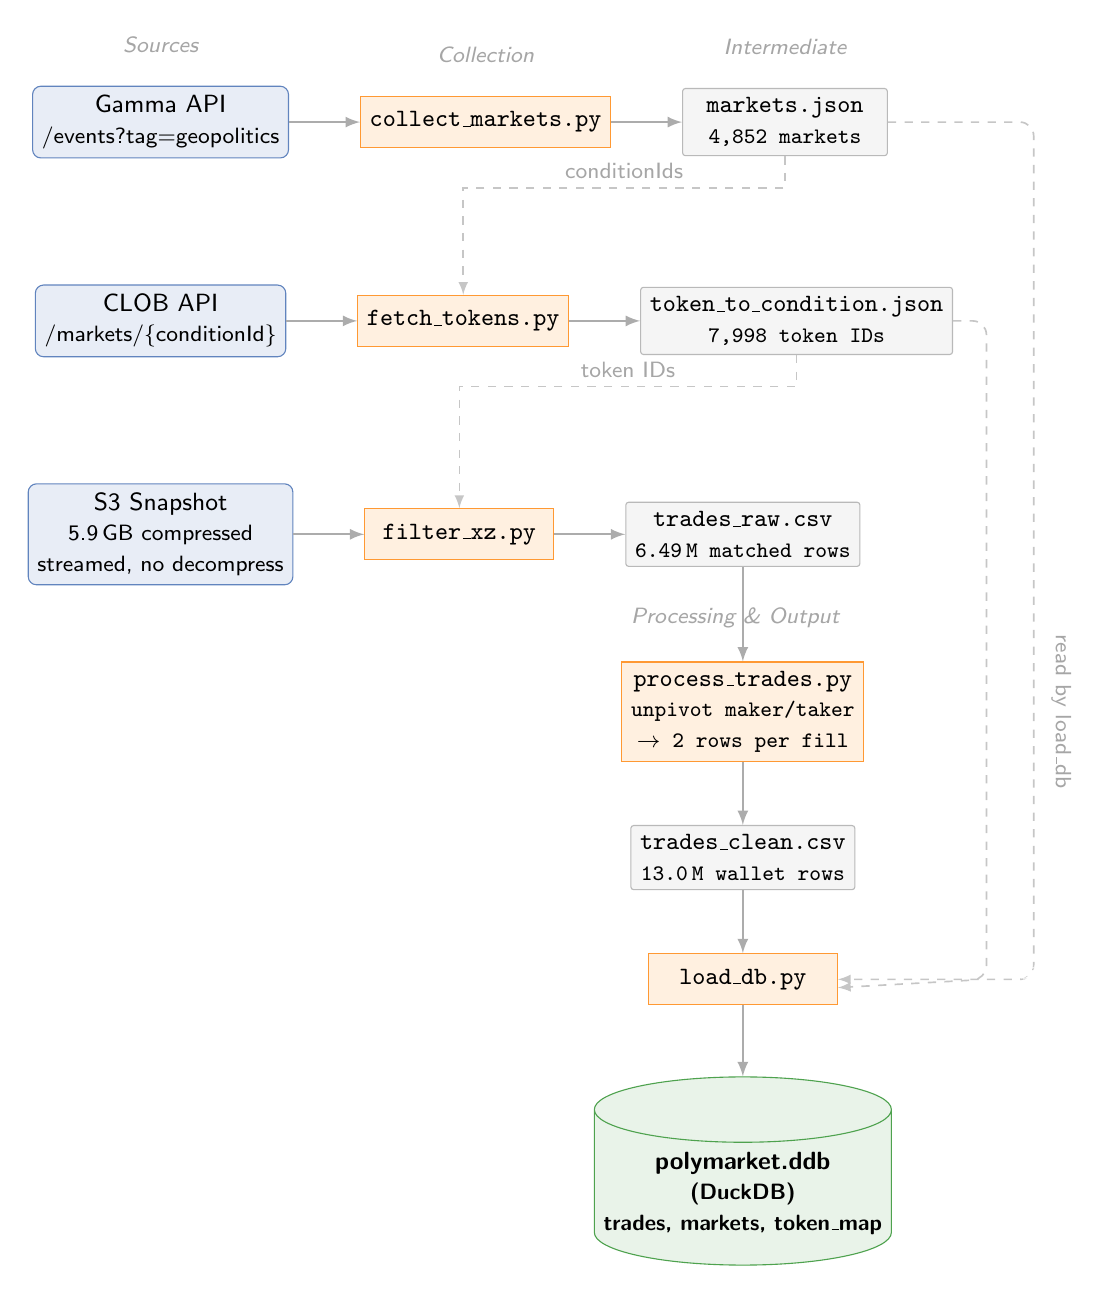
\begin{tikzpicture}[
    node distance = 0.6cm and 0.9cm,
    % ── Node styles ──
    api/.style   = {rectangle, rounded corners=3pt,
                    draw=PolyBlue!70, fill=PolyBlue!10,
                    minimum width=2.4cm, minimum height=0.7cm,
                    font=\small\sffamily, align=center},
    script/.style= {rectangle,
                    draw=orange!80, fill=orange!12,
                    minimum width=2.4cm, minimum height=0.65cm,
                    font=\small\ttfamily, align=center},
    file/.style  = {rectangle, rounded corners=1pt,
                    draw=gray!55, fill=gray!8,
                    minimum width=2.6cm, minimum height=0.65cm,
                    font=\small\ttfamily, align=center},
    db/.style    = {cylinder, shape border rotate=90, aspect=0.22,
                    draw=ForestGreen!80, fill=ForestGreen!10,
                    minimum width=2.6cm, minimum height=0.9cm,
                    font=\small\sffamily\bfseries, align=center},
    arr/.style   = {->, >=latex, thick, gray!65},
    dep/.style   = {->, >=latex, semithick, gray!45, dashed},
    arrlbl/.style= {font=\footnotesize\sffamily, text=gray!70, fill=white, inner sep=2pt},
    labl/.style  = {font=\footnotesize\sffamily\itshape, text=gray!70},
]

% =====================================================================
%  ROW 1: Gamma API → collect_markets.py → markets.json
% =====================================================================
\node[api] (gamma) {Gamma API\\
    {\footnotesize /events?tag=geopolitics}};
\node[script, right=0.9cm of gamma] (cm) {collect\_markets.py};
\node[file, right=0.9cm of cm] (mj) {markets.json\\
    {\footnotesize 4{,}852 markets}};

\draw[arr] (gamma) -- (cm);
\draw[arr] (cm)    -- (mj);

% =====================================================================
%  ROW 2: CLOB API → fetch_tokens.py → token_to_condition.json
% =====================================================================
\node[api, below=1.6cm of gamma] (clob) {CLOB API\\
    {\footnotesize /markets/\{conditionId\}}};
\node[script, right=0.9cm of clob] (ft) {fetch\_tokens.py};
\node[file, right=0.9cm of ft] (tc) {token\_to\_condition.json\\
    {\footnotesize 7{,}998 token IDs}};

\draw[arr] (clob) -- (ft);
\draw[arr] (ft)   -- (tc);

% ── markets.json → fetch_tokens (conditionIds flow down)
\draw[dep] (mj.south) -- ++(0,-0.4) coordinate (cid-horiz) -| (ft.north);
\node[arrlbl, above=1pt] at ($(cid-horiz)!0.5!(cid-horiz -| ft.north)$) {conditionIds};

% =====================================================================
%  ROW 3: S3 Snapshot → filter_xz.py → trades_raw.csv
% =====================================================================
\node[api, below=1.6cm of clob] (s3) {S3 Snapshot\\
    {\footnotesize 5.9\,GB compressed}\\
    {\footnotesize streamed, no decompress}};
\node[script, right=0.9cm of s3] (fx) {filter\_xz.py};
\node[file, right=0.9cm of fx] (tr) {trades\_raw.csv\\
    {\footnotesize 6.49\,M matched rows}};

\draw[arr] (s3) -- (fx);
\draw[arr] (fx) -- (tr);

% ── token_to_condition → filter_xz (token IDs flow down)
\draw[dep] (tc.south) -- ++(0,-0.4) coordinate (tid-horiz) -| (fx.north);
\node[arrlbl, above=1pt] at ($(tid-horiz)!0.5!(tid-horiz -| fx.north)$) {token IDs};

% =====================================================================
%  VERTICAL CASCADE: process → clean → load → DuckDB
%  Centred under the Intermediate column
% =====================================================================

% ── process_trades.py
\node[script, below=1.2cm of tr] (pt) {process\_trades.py\\
    {\footnotesize unpivot maker/taker}\\
    {\footnotesize $\rightarrow$ 2 rows per fill}};
\draw[arr] (tr.south) -- (pt.north);

% ── trades_clean.csv
\node[file, below=0.8cm of pt] (tc2) {trades\_clean.csv\\
    {\footnotesize 13.0\,M wallet rows}};
\draw[arr] (pt.south) -- (tc2.north);

% ── load_db.py
\node[script, below=0.8cm of tc2] (ld) {load\_db.py};
\draw[arr] (tc2.south) -- (ld.north);

% ── DuckDB
\node[db, below=0.9cm of ld] (ddb) {polymarket.ddb\\
    {\footnotesize (DuckDB)}\\
    {\footnotesize trades, markets, token\_map}};
\draw[arr] (ld.south) -- (ddb.north);

% =====================================================================
%  RIGHT-SIDE RAIL: markets.json & token_map also feed load_db
%  Use a single vertical rail at x = right edge of diagram
% =====================================================================
\coordinate (rail) at ([xshift=2.2cm]tr.east);

% markets.json → load_db (via rail)
\draw[dep, rounded corners=5pt]
    (mj.east) -- (mj.east -| rail) -- (rail |- ld.east) -- (ld.east)
    node[arrlbl, pos=0.0, above right, xshift=-4pt] {};

% token_to_condition → load_db (via rail, offset slightly)
\coordinate (rail2) at ([xshift=1.6cm]tr.east);
\draw[dep, rounded corners=5pt]
    (tc.east) -- (tc.east -| rail2) -- (rail2 |- ld.east) -- ([yshift=-3pt]ld.east);

% ── Annotations on rail
\node[arrlbl, rotate=-90, anchor=south] at ([xshift=0.15cm]rail |- pt) 
    {read by load\_db};

% =====================================================================
%  COLUMN LABELS
% =====================================================================
\node[labl, above=0.3cm of gamma] {Sources};
\node[labl, above=0.3cm of cm]    {Collection};
\node[labl, above=0.3cm of mj]    {Intermediate};
\node[labl, above=0.3cm of pt.north west, anchor=south west] {Processing \& Output};

\end{tikzpicture}
\caption{Data collection and loading pipeline. Orange: Python scripts
         (\texttt{src/pipeline/}), blue: external data sources, grey:
         intermediate files, green: analytical database.
         Solid arrows show the primary data flow; dashed arrows show
         secondary dependencies (metadata lookups).
         \texttt{filter\_xz.py} streams the S3 snapshot without full
         decompression, matching token IDs on the fly.
         Full pipeline reproducible via \texttt{make pipeline}.}
\label{fig:pipeline}
\end{figure}


\newpage

\subsubsection*{Step 0: S3 Snapshot Download:}

The first step is downloading \texttt{orderFilled\_complete.csv.xz}
into \texttt{data/raw/} from the \texttt{warproxxx/poly\_data} S3
archive (see Appendix~\ref{app:download}).

\begin{table}[H]
\centering
\caption{Example rows from \texttt{orderFilled\_complete.csv.xz}.
         Each trade assets are identified by ERC-1155 token IDs, these are
         77-digit integers assigned at market creation, one for both Yes and No.\texttt{0} denotes USDC. 
         No condition IDs or market names are present in
         the raw data, therefore the following steps of the pipeline exist to resolve this problem.}
\label{tab:raw_snapshot}
\small
\begin{tabularx}{\textwidth}{l l l r l r}
\toprule
\textbf{timestamp} & \textbf{maker} & \textbf{makerAssetId}
    & \textbf{makerAmt} & \textbf{takerAssetId} & \textbf{takerAmt} \\
\midrule
1675247746 & \texttt{0x78db{\ldots}} & \texttt{0} (USDC)
    & 29.68 & \texttt{55628{\ldots}} & 30.60 \\
1675247746 & \texttt{0xc6fd{\ldots}} & \texttt{41572{\ldots}}
    & 30.60 & \texttt{0} (USDC) & 0.92 \\
\bottomrule
\end{tabularx}
\end{table}


% ── Step 1 ────────────────────────────────────────────────────────────────────
\subsubsection*{Step 1: \texttt{collect\_markets.py}}
The pipeline begins by querying the Gamma API for all closed geopolitical markets, paginating until exhausted, and writes the result to \texttt{data/raw/markets.json}.
This file serves as the master market registry all over steps.

\lstinputlisting[
    language=Python,
    firstline=16, lastline=19,
    caption={Gamma API query parameters.},
    label={lst:collect_markets}
]{../src/pipeline/collect_markets.py}

\texttt{resolvedOutcome} is not returned directly by the API, it is 
derived by parsing the \texttt{outcomePrices}, string into a list and 
selecting the outcome where the price goes to \$1 at settlement. Over 5000 markets were retrieved with these parameters as of April 2026. The following table summarises the markets.json schema:

\begin{table}[H]
\centering
\caption{\texttt{markets.json} field reference.}
\label{tab:markets_schema}
\small
\begin{tabularx}{\textwidth}{l l X}
\toprule
\textbf{Field} & \textbf{Type} & \textbf{Example} \\
\midrule
\texttt{conditionId}     & string   & \texttt{0x0f99\ldots} \\
\texttt{question}        & string   & Will Putin remain President through 2024? \\
\texttt{eventTitle}      & string   & Will Putin remain President through 2024? \\
\texttt{startDate}       & ISO 8601 & \texttt{2024-03-26T15:11:43Z} \\
\texttt{endDate}         & ISO 8601 & \texttt{2024-12-31T12:00:00Z} \\
\texttt{closedTime}      & ISO 8601 & \texttt{2025-01-01T09:42:22Z} \\
\texttt{volume}          & float    & \texttt{2{,}187{,}634} \\
\texttt{outcomes}        & string[] & \texttt{["Yes", "No"]} \\
\texttt{outcomePrices}   & string[] & \texttt{["1", "0"]} \\
\texttt{resolvedOutcome} & string   & \texttt{Yes} (derived from \texttt{outcomePrices}) \\
\texttt{tags}            & string[] & \texttt{["russia", "putin", "geopolitics", \ldots]} \\
\bottomrule
\end{tabularx}
\end{table}





\subsubsection*{Step 2 \texttt{fetch\_tokens.py}}

As shown in Table~\ref{tab:raw_snapshot}, snapshot rows carry no 
conditionID (cid), only ERC-1155 token IDs. \texttt{fetch\_tokens.py} 
resolves this by querying the CLOB API for the YES/NO ERC-1155 token IDs of 
each market in \texttt{markets.json} with volume $\geq$\$1{,}000. 

\begin{figure}[H]
\centering
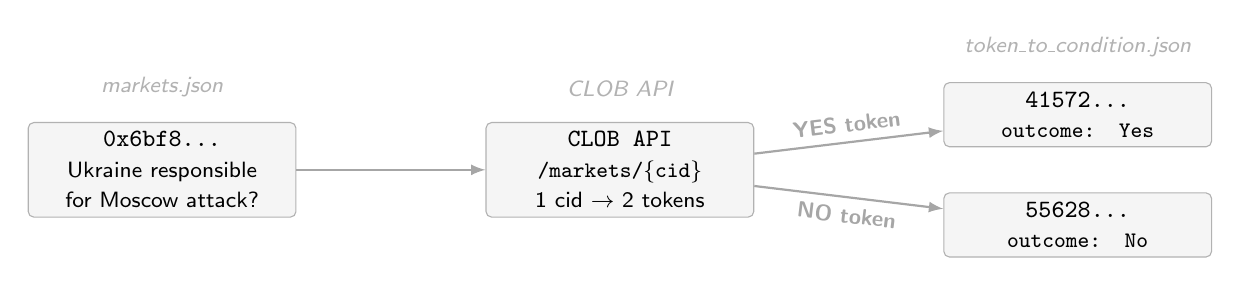
\begin{tikzpicture}[
    box/.style={rectangle, draw=gray!60, fill=gray!8, 
                rounded corners=2pt, minimum width=3.4cm, 
                minimum height=0.75cm, font=\small\ttfamily, align=center},
    arr/.style={->, >=latex, thick, gray!70},
    lbl/.style={font=\footnotesize\sffamily\itshape, text=gray!60},
    side/.style={font=\footnotesize\sffamily\bfseries, text=gray!70}
]

\node[box] (cid)  
    {\texttt{0x6bf8\ldots}\\
     {\footnotesize\sffamily Ukraine responsible}\\
     {\footnotesize\sffamily for Moscow attack?}};

\node[box, right=2.4cm of cid] (clob) 
    {CLOB API\\{\footnotesize /markets/\{cid\}}\\
     {\footnotesize\sffamily 1 cid $\rightarrow$ 2 tokens}};

\node[box, right=2.4cm of clob, yshift=0.7cm] (yes)  
    {\texttt{41572\ldots}\\{\footnotesize outcome: \textbf{Yes}}};

\node[box, right=2.4cm of clob, yshift=-0.7cm] (no)   
    {\texttt{55628\ldots}\\{\footnotesize outcome: \textbf{No}}};

\draw[arr] (cid)  -- (clob);
\draw[arr] (clob) -- node[side, above, sloped] {YES token} (yes);
\draw[arr] (clob) -- node[side, below, sloped] {NO token}  (no);

\node[lbl, above=0.2cm of cid]  {markets.json};
\node[lbl, above=0.2cm of clob] {CLOB API};
\node[lbl, above=0.2cm of yes]  {token\_to\_condition.json};

\end{tikzpicture}
\caption{Each \texttt{conditionId} is resolved to a YES and NO 
ERC-1155 token ID via the CLOB API. The token IDs shown are real 
values from the dataset.}
\label{fig:token_mapping}
\end{figure}

\noindent The \$1{,}000 volume filter excludes negligible markets,
at time of writing, \texttt{token\_to\_condition.json} contained
approximately 8,000 token IDs across 4,000 markets.





\newpage

\subsubsection*{Step 3: \texttt{filter\_xz.py}}

Using the token to condition mapping, the \texttt{filter\_xz.py} extracts matching trades from the full snapshot in a single streaming pass.
Full decompression is impractical, given the archive size
at 35-40\,GB (Table~\ref{tab:s3_snapshot}). 
\texttt{xzcat}\footnote{\url{https://linux.die.net/man/1/xzcat}} (Unix utility) is used to stream the \texttt{.xz} file line by line into a Python CSV reader, without having to write the full decompressed file to disk. 

\begin{lstlisting}[language=Python, caption={Streaming the \texttt{.xz} archive without full decompression.}, label={lst:filter_xz}]
with subprocess.Popen(["xzcat", str(IN)], 
                      stdout=subprocess.PIPE, 
                      bufsize=1024*1024) as proc:
    reader = csv.reader(line.decode() for line in proc.stdout)
\end{lstlisting}

\noindent Each row is checked against \texttt{token\_to\_condition.json}:
a match on either \texttt{makerAssetId} or \texttt{takerAssetId} means the row is written to the .csv file, with \texttt{condition\_id} and \texttt{outcomes} appended to that output row.

\begin{table}[H]
\centering
\caption{\texttt{trades\_raw.csv} - output of \texttt{filter\_xz.py}.}
\label{tab:trades_raw}
\small
\begin{tabularx}{\textwidth}{l X}
\toprule
\textbf{Property} & \textbf{Value} \\
\midrule
Rows           & 6,505,297 ($\approx4.3\%$ of full snapshot) \\
Unique wallets & 333,124 \\
File size      & 2.1\,GB \\
Date range     & 1 February 2023 - 7 October 2025 \\
Added columns  & \texttt{condition\_id}, \texttt{outcomes} \\
\bottomrule
\end{tabularx}
\end{table}










\subsubsection*{Step 4 \texttt{process\_trades.py}}


% TODO: INCLUDE THIS SNIPPET OR APPENDIX maker_is_buyer = row["makerAssetId"] == "0"
Each raw fill in \texttt{trades\_raw.csv} records both the maker and
taker in a single row. \texttt{process\_trades.py} normalises this into
wallet-centric rows suitable analysis:

\begin{itemize}
    \item \textbf{Unpivot:} Each fill is split into two rows, a taker and a maker since every trade has exactly one buyer and seller. This expends the 6.5\,M fills to 13.0\,M wallet-centric rows.
    \item \textbf{Side inference:} For each \texttt{OrderFilled} event, 
          the maker places the limit order and the taker fills it. When
          \texttt{makerAssetId} $= 0$ this indicates the maker paid USDC to 
          acquire outcome tokens (\texttt{BUY}). Otherwise the maker 
          delivered outcome tokens to receive USDC (\texttt{SELL}).
    \item \textbf{Normalisation:} raw integer amounts are divided by 
          $10^6$ to convert from ERC-1155 precision to USDC and token units
    \item \textbf{Price:} derived as $\texttt{price} = \texttt{usd\_amount} 
          / \texttt{token\_amount}$, representing the implied probability 
          at time of trade.
    \item \textbf{Dust filter:} rows where the normalised token amount 
          rounds to zero are discarded completely.
\end{itemize}

\begin{table}[H]
\centering
\caption{Sample rows from \texttt{trades\_clean.csv}. Each original
         fill becomes two rows with opposite sides.}
\label{tab:clean_sample}
\small
\begin{tabularx}{\textwidth}{l l l l r r r}
\toprule
\textbf{timestamp} & \textbf{wallet} & \textbf{side} &
\textbf{outcome} & \textbf{usd} & \textbf{tokens} & \textbf{price} \\
\midrule
2023-02-01 & \texttt{0x78db{\ldots}} & BUY  & No  & 29.68 & 30.60 & 0.97 \\
2023-02-01 & \texttt{0x4bfb{\ldots}} & SELL & No  & 29.68 & 30.60 & 0.97 \\
2023-02-01 & \texttt{0xc6fd{\ldots}} & BUY  & Yes &  0.92 & 30.60 & 0.03 \\
2023-02-01 & \texttt{0x78db{\ldots}} & SELL & Yes &  0.92 & 30.60 & 0.03 \\
\bottomrule
\end{tabularx}
\end{table}


  
\subsubsection*{Step 5: \texttt{load\_db.py}}

\texttt{load\_db.py} is the final step of the core pipeline, loading the
\texttt{trades\_clean.csv} and \texttt{markets.json} into a single
DuckDB analytical database (\texttt{polymarket.ddb}).
Unix timestamps are converted into native \texttt{TIMESTAMP} columns, the
\texttt{tags} field is converted from a raw JSON string to a native
\texttt{VARCHAR[]} array.
The token map is kept as a \texttt{token\_map} table for possible future
cross-reference.
The resulting schema, and the database choice of DuckDB, are covered in Section~\ref{sec:schema}.


% ── 2.3 Database Schema ───────────────────────────────────────────────────────
\subsection{Database Schema}
\label{sec:schema}

All pipeline outputs are merged into a single DuckDB
database (\texttt{polymarket.ddb}).  DuckDB was chosen for three main reasons~\cite{duckdb}:

\begin{itemize}
    \item \textbf{Columnar execution:} its vectorised engine handles
          time-series aggregations and \texttt{GROUP BY} queries more efficiently than a row-oriented store such as SQLite, especially across 13 million wallet rows. 
    \item \textbf{Native array support:} the \texttt{VARCHAR[]} type
          allows market tags to be stored and filtered directly, removing
          the need for a separate junction table.
    \item \textbf{Serverless:} like SQLite, no background process is needed, keeping
          the database fully portable as a single file within the project
          repository.
\end{itemize}

\noindent The database contains five tables, summarised in
Table~\ref{tab:rowcounts}.  Three are loaded by the core pipeline
(\texttt{load\_db.py}): \texttt{trades}, \texttt{markets}, and
\texttt{token\_map}.  Two further tables, \texttt{sentiment} and
\texttt{financial} are both populated by the sentiment pipeline
(Section~\ref{sec:sentiment}) and joined to the core tables by the shared foreign key,
\texttt{condition\_id}.

\begin{table}[H]
\centering
\caption{Database tables after the full pipeline.}
\label{tab:rowcounts}
\small
\begin{tabularx}{\textwidth}{l r X}
\toprule
\textbf{Table} & \textbf{Rows} & \textbf{Loaded by} \\
\midrule
\texttt{trades}     & 13{,}010{,}594 & \texttt{load\_db.py} \\
\texttt{markets}    &      5{,}372   & \texttt{load\_db.py} \\
\texttt{token\_map} &      8{,}794   & \texttt{load\_db.py} \\
\texttt{sentiment}  &        ---     & sentiment pipeline
                                       (Section~\ref{sec:sentiment}) \\
\texttt{financial}  &        ---     & sentiment pipeline
                                       (Section~\ref{sec:sentiment}) \\
\bottomrule
\end{tabularx}
\end{table}

\noindent Figure \ref{fig:schema} shows the full schema and
relationships between tables.  \texttt{condition\_id} is the shared
foreign key that links trade activity, market metadata, token
identifiers, and the sentiment and financial enrichment layers.

% ── Schema diagram ───────────────────────────────────────────────────────────
\begin{figure}[H]
\centering
\resizebox{\textwidth}{!}{%
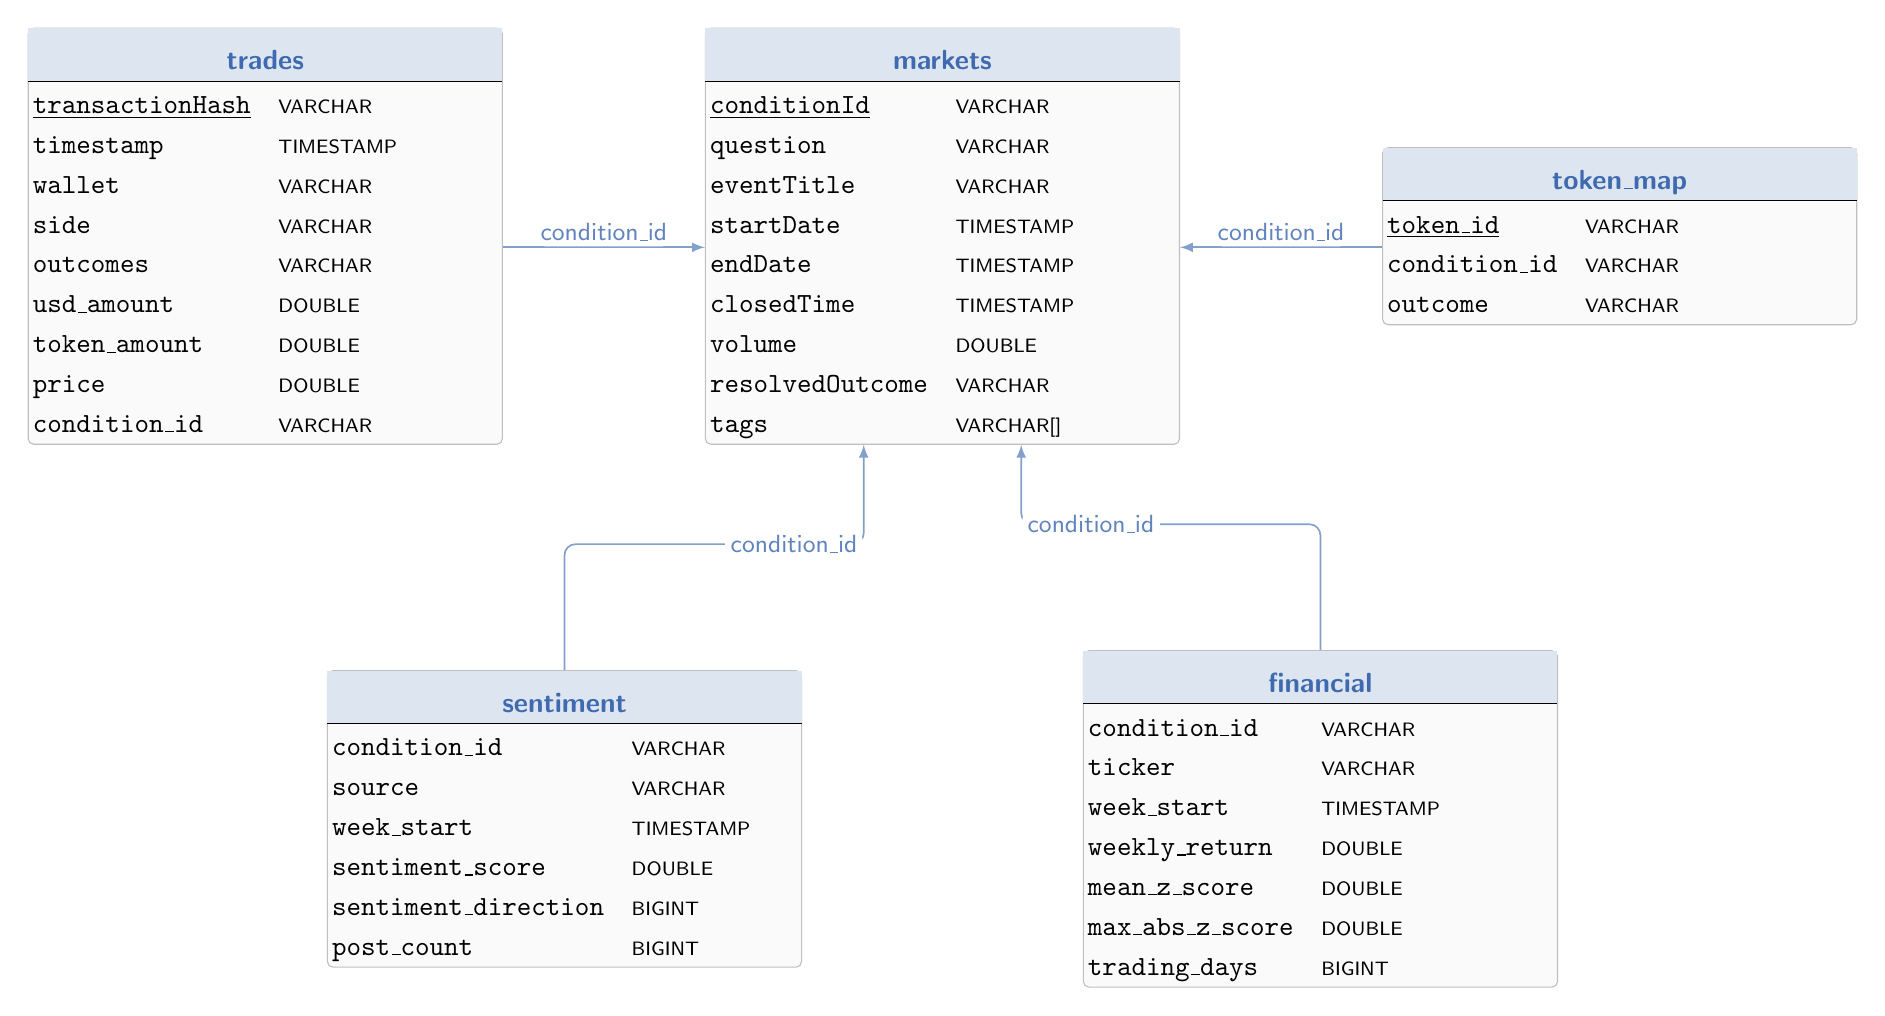
\begin{tikzpicture}[
    fk/.style    = {->, >=latex, semithick, PolyBlue!55},
    fklbl/.style = {font=\small\sffamily, text=PolyBlue!70,
                    fill=white, inner sep=2pt},
]
 
% =====================================================================
%  MARKETS  (top-centre — the hub)
% =====================================================================
\node[draw=gray!50, fill=gray!4, inner sep=0pt, rounded corners=2pt]
    (markets) at (0, 0) {%
    \begin{tabular}{@{\,}l@{\hskip 10pt}l@{\,}}
      \multicolumn{2}{c}{%
        \cellcolor{PolyBlue!15}%
        \makebox[5.6cm][c]{\rule{0pt}{1.5em}%
          \textsf{\textbf{\textcolor{PolyBlue!85}{markets}}}}}\\[-0.4pt]
      \hline \rule{0pt}{1.15em}%
      \underline{\texttt{conditionId}}     & \textsf{\scriptsize VARCHAR}   \\
      \texttt{question}                    & \textsf{\scriptsize VARCHAR}   \\
      \texttt{eventTitle}                  & \textsf{\scriptsize VARCHAR}   \\
      \texttt{startDate}                   & \textsf{\scriptsize TIMESTAMP} \\
      \texttt{endDate}                     & \textsf{\scriptsize TIMESTAMP} \\
      \texttt{closedTime}                  & \textsf{\scriptsize TIMESTAMP} \\
      \texttt{volume}                      & \textsf{\scriptsize DOUBLE}    \\
      \texttt{resolvedOutcome}             & \textsf{\scriptsize VARCHAR}   \\
      \texttt{tags}                        & \textsf{\scriptsize VARCHAR[]} \\
    \end{tabular}%
};
 
% =====================================================================
%  TRADES  (left of markets)
% =====================================================================
\node[draw=gray!50, fill=gray!4, inner sep=0pt, rounded corners=2pt]
    (trades) at (-8.6, 0) {%
    \begin{tabular}{@{\,}l@{\hskip 10pt}l@{\,}}
      \multicolumn{2}{c}{%
        \cellcolor{PolyBlue!15}%
        \makebox[5.6cm][c]{\rule{0pt}{1.5em}%
          \textsf{\textbf{\textcolor{PolyBlue!85}{trades}}}}}\\[-0.4pt]
      \hline \rule{0pt}{1.15em}%
      \underline{\texttt{transactionHash}} & \textsf{\scriptsize VARCHAR}   \\
      \texttt{timestamp}                   & \textsf{\scriptsize TIMESTAMP} \\
      \texttt{wallet}                      & \textsf{\scriptsize VARCHAR}   \\
      \texttt{side}                        & \textsf{\scriptsize VARCHAR}   \\
      \texttt{outcomes}                    & \textsf{\scriptsize VARCHAR}   \\
      \texttt{usd\_amount}                 & \textsf{\scriptsize DOUBLE}    \\
      \texttt{token\_amount}               & \textsf{\scriptsize DOUBLE}    \\
      \texttt{price}                       & \textsf{\scriptsize DOUBLE}    \\
      \textbf{\texttt{condition\_id}}      & \textsf{\scriptsize VARCHAR}   \\
    \end{tabular}%
};
 
% =====================================================================
%  TOKEN_MAP  (right of markets)
% =====================================================================
\node[draw=gray!50, fill=gray!4, inner sep=0pt, rounded corners=2pt]
    (tokenmap) at (8.6, 0) {%
    \begin{tabular}{@{\,}l@{\hskip 10pt}l@{\,}}
      \multicolumn{2}{c}{%
        \cellcolor{PolyBlue!15}%
        \makebox[5.6cm][c]{\rule{0pt}{1.5em}%
          \textsf{\textbf{\textcolor{PolyBlue!85}{token\_map}}}}}\\[-0.4pt]
      \hline \rule{0pt}{1.15em}%
      \underline{\texttt{token\_id}}       & \textsf{\scriptsize VARCHAR} \\
      \textbf{\texttt{condition\_id}}      & \textsf{\scriptsize VARCHAR} \\
      \texttt{outcome}                     & \textsf{\scriptsize VARCHAR} \\
    \end{tabular}%
};
 
% =====================================================================
%  SENTIMENT  (bottom-left)
% =====================================================================
\node[draw=gray!50, fill=gray!4, inner sep=0pt, rounded corners=2pt]
    (sentiment) at (-4.8, -7.4) {%
    \begin{tabular}{@{\,}l@{\hskip 10pt}l@{\,}}
      \multicolumn{2}{c}{%
        \cellcolor{PolyBlue!15}%
        \makebox[5.6cm][c]{\rule{0pt}{1.5em}%
          \textsf{\textbf{\textcolor{PolyBlue!85}{sentiment}}}}}\\[-0.4pt]
      \hline \rule{0pt}{1.15em}%
      \textbf{\texttt{condition\_id}}      & \textsf{\scriptsize VARCHAR}   \\
      \texttt{source}                      & \textsf{\scriptsize VARCHAR}   \\
      \texttt{week\_start}                 & \textsf{\scriptsize TIMESTAMP} \\
      \texttt{sentiment\_score}            & \textsf{\scriptsize DOUBLE}    \\
      \texttt{sentiment\_direction}        & \textsf{\scriptsize BIGINT}    \\
      \texttt{post\_count}                 & \textsf{\scriptsize BIGINT}    \\
    \end{tabular}%
};
 
% =====================================================================
%  FINANCIAL  (bottom-right)
% =====================================================================
\node[draw=gray!50, fill=gray!4, inner sep=0pt, rounded corners=2pt]
    (financial) at (4.8, -7.4) {%
    \begin{tabular}{@{\,}l@{\hskip 10pt}l@{\,}}
      \multicolumn{2}{c}{%
        \cellcolor{PolyBlue!15}%
        \makebox[5.6cm][c]{\rule{0pt}{1.5em}%
          \textsf{\textbf{\textcolor{PolyBlue!85}{financial}}}}}\\[-0.4pt]
      \hline \rule{0pt}{1.15em}%
      \textbf{\texttt{condition\_id}}      & \textsf{\scriptsize VARCHAR}   \\
      \texttt{ticker}                      & \textsf{\scriptsize VARCHAR}   \\
      \texttt{week\_start}                 & \textsf{\scriptsize TIMESTAMP} \\
      \texttt{weekly\_return}              & \textsf{\scriptsize DOUBLE}    \\
      \texttt{mean\_z\_score}              & \textsf{\scriptsize DOUBLE}    \\
      \texttt{max\_abs\_z\_score}          & \textsf{\scriptsize DOUBLE}    \\
      \texttt{trading\_days}               & \textsf{\scriptsize BIGINT}    \\
    \end{tabular}%
};
 
% =====================================================================
%  FK ARROWS — all point inward to markets.conditionId
% =====================================================================
 
% trades.condition_id → markets.conditionId
\draw[fk, rounded corners=4pt]
    ([yshift=-4pt]trades.east) -- ([yshift=-4pt]markets.west)
    node[fklbl, midway, above] {condition\_id};
 
% token_map.condition_id → markets.conditionId
\draw[fk, rounded corners=4pt]
    ([yshift=-4pt]tokenmap.west) -- ([yshift=-4pt]markets.east)
    node[fklbl, midway, above] {condition\_id};
 
% sentiment.condition_id → markets.conditionId
\draw[fk, rounded corners=4pt]
    (sentiment.north) -- ++(0, 1.6)
    -| ([xshift=-1.0cm]markets.south)
    node[fklbl, pos=0.50, left] {condition\_id};
 
% financial.condition_id → markets.conditionId
\draw[fk, rounded corners=4pt]
    (financial.north) -- ++(0, 1.6)
    -| ([xshift=1.0cm]markets.south)
    node[fklbl, pos=0.50, right] {condition\_id};
 
\end{tikzpicture}%
}% end resizebox
\caption{Database schema.  Underlined fields denote primary keys;
         bold fields are foreign keys referencing
         \texttt{markets.conditionId}.  The \texttt{sentiment} and
         \texttt{financial} tables are populated by the sentiment
         pipeline (Section~\ref{sec:sentiment}).}
\label{fig:schema}
\end{figure}

\noindent An exploratory analysis of the resulting dataset, covering
wallet activity distributions, volume concentration, hit rates, and
market coverage-is provided in Section \ref{sec:eda}.



\newpage

\newpage
% ==========================================================
%  SECTION 3 - SENTIMENT AND FINANCIAL SIGNAL PIPELINE
% ==========================================================
% ==========================================================
%  SECTION 3 - SENTIMENT AND FINANCIAL SIGNAL PIPELINE
% ==========================================================
\section{Sentiment and Financial Signal Pipeline}
\label{sec:sentiment}

The trade data from Section~\ref{sec:pipeline} records wallet
activity, but not the information environment in which each trade
was placed. 
A trade viewed completely in isolation is ambiguous,  a YES position
on a resolved market could reflect anything from luck to a reasonable read of public
news to possible access to information not yet reflected in price. 
To attempt to separate these cases, each trade must be set against the external
signals available during the same week.

\hspace{1cm}Table~\ref{tab:signal_motivation} illustrates this with a real
market. On 3 April 2025, a wallet buys YES on an Iran-Israel strike
market at \$0.12, against an information environment that was
broadly sceptical. The strike occurs ten days later and the position
resolves at \$1.00. Without the surrounding context, the trade is
indistinguishable from a lucky  bet but  with some extra context, the wallets deviation from the
public consensus become more measurable.

\begin{table}[H]
\centering
\caption{A single trade against its weekly information environment.
         The wallet enters at \$0.12 during a week when all three
         external signals lean against the YES outcome; the market
         resolves YES ten days later. Signal values are illustrative.}
\label{tab:signal_motivation}
\small
\begin{tabularx}{\textwidth}{l l l X}
\toprule
\textbf{Signal} & \textbf{Score} & \textbf{Volume} & \textbf{Interpretation} \\
\midrule
FT / FinBERT            & $-0.42$ & 8 articles & Coverage emphasises diplomatic de-escalation \\
Truth Social / VADER    & $+0.05$ & 2 posts    & Neutral; no direct reference to Iran \\
IDF defence basket      & $-0.30$ & ---        & No abnormal move \\
\midrule
\multicolumn{4}{l}{\textbf{Trade:} wallet \texttt{0x78db\ldots} buys YES at \$0.12 on 2025-04-03 (week of 2025-03-31 to 2025-04-06)} \\
\multicolumn{4}{l}{\textbf{Resolution:} YES settles at \$1.00 on 2025-04-13} \\
\bottomrule
\end{tabularx}
\end{table}

\noindent This is the pattern the enrichment layer exists to surface:
a wallet taking a position against these signals and
being proven right. 
This looked at in more depth in Section~\ref{sec:signal_analysis}.

The remainder of this section describes the three sources. Each is
aggregated to weekly resolution and keyed on \texttt{condition\_id}
+ \texttt{week\_start}:

\begin{itemize}
    \item \textbf{Elite financial discourse.} Financial Times
          articles scored with FinBERT \cite{araci2019finbert}.
    \item \textbf{Executive political discourse.} Donald Trump's
          Truth Social posts scored with VADER \cite{hutto2014vader},
          sourced from
          \texttt{stiles/trump-truth-social-archive}
          \cite{trump_archive}.
    \item \textbf{Market-implied consensus.} yfinance daily OHLCV
          for geopolitically-linked tickers, converted to weekly
          abnormal returns against a 20-day rolling baseline, with
          CBOE VIX as a global volatility benchmark.
\end{itemize}

\noindent Signals are joined at the week a wallet enters a
market, not at resolution date. 
A bet with possible extra information might be placed months
before the market closes, if the signals are only looked up at the 
resolution date, the rest of the market's life and the wallet's position would not be counted for. 

% ── 3.1 Architecture Overview ────────────────────────────────────────────────
\subsection{Architecture Overview}
\label{sec:sentiment_architecture}

Figure~\ref{fig:sentiment_pipeline} shows the three parallel tracks
that produce the enrichment tables. All three consume the shared
\texttt{markets} table and NER module, and all three write into the
same \texttt{polymarket.ddb} database established in
Section~\ref{sec:pipeline}. A single vocabulary module,
\texttt{pipeline\_config.py}, drives keyword-to-corpus, keyword-to-ticker,
and author-stopword mappings across all three collectors — covered
in the subsections that follow.

\begin{figure}[H]
\centering
\resizebox{\textwidth}{!}{%
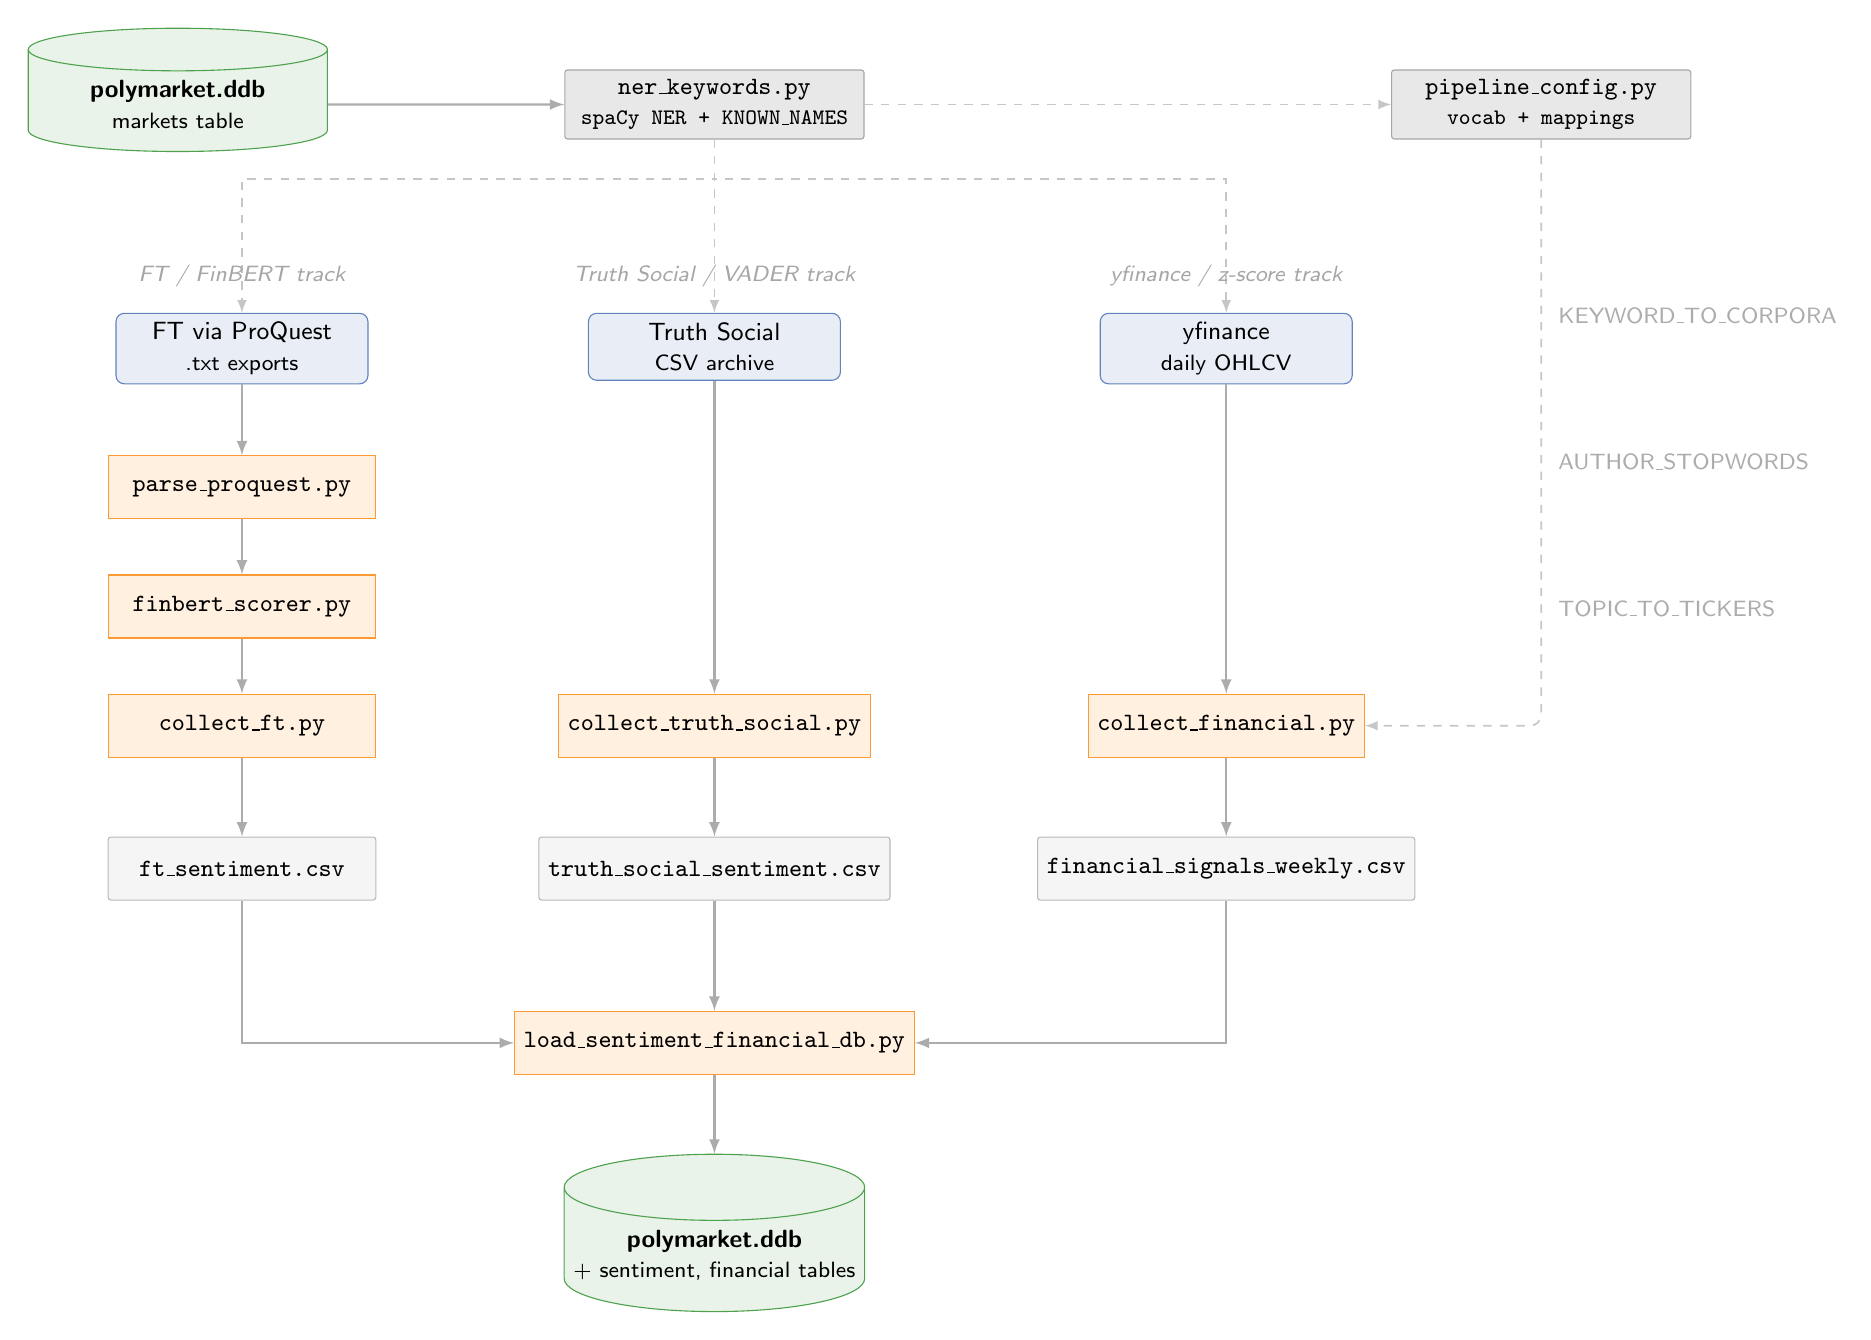
\begin{tikzpicture}[
    node distance = 0.7cm and 1.5cm,
    % ── Node styles (match Figure 1) ──
    api/.style   = {rectangle, rounded corners=3pt,
                    draw=PolyBlue!70, fill=PolyBlue!10,
                    minimum width=3.2cm, minimum height=0.85cm,
                    font=\small\sffamily, align=center},
    script/.style= {rectangle,
                    draw=orange!80, fill=orange!12,
                    minimum width=3.4cm, minimum height=0.8cm,
                    font=\small\ttfamily, align=center},
    file/.style  = {rectangle, rounded corners=1pt,
                    draw=gray!55, fill=gray!8,
                    minimum width=3.4cm, minimum height=0.8cm,
                    font=\small\ttfamily, align=center},
    shared/.style= {rectangle, rounded corners=1pt,
                    draw=gray!70, fill=gray!18,
                    minimum width=3.8cm, minimum height=0.85cm,
                    font=\small\ttfamily\bfseries, align=center},
    db/.style    = {cylinder, shape border rotate=90, aspect=0.22,
                    draw=ForestGreen!80, fill=ForestGreen!10,
                    minimum width=3.8cm, minimum height=1.1cm,
                    font=\small\sffamily\bfseries, align=center},
    arr/.style   = {->, >=latex, thick, gray!65},
    dep/.style   = {->, >=latex, semithick, gray!45, dashed},
    labl/.style  = {font=\footnotesize\sffamily\itshape, text=gray!70},
    deplbl/.style= {font=\footnotesize\sffamily, text=gray!65,
                    fill=white, inner sep=2pt},
]

% =====================================================================
%  ROW 0 : shared inputs
% =====================================================================
\node[db] (markets) at (0,0) {polymarket.ddb\\
    {\footnotesize\mdseries markets table}};

\node[shared, right=3.0cm of markets] (ner)
    {ner\_keywords.py\\
    {\footnotesize\mdseries spaCy NER + KNOWN\_NAMES}};

% pipeline_config now sits directly above where collect_financial.py will be
% fin_src is at xshift=6.5cm of ner (row 1), so match that x position
\node[shared] (config) at ($(ner) + (10.5cm, 0)$)
    {pipeline\_config.py\\
    {\footnotesize\mdseries vocab + mappings}};

\draw[arr] (markets) -- (ner);

% NER depends on pipeline_config
\draw[dep] (ner) -- (config);

% =====================================================================
%  ROW 1 : external sources
% =====================================================================
\node[api, below=2.2cm of ner, xshift=-6.0cm] (ft_src)
    {FT via ProQuest\\{\footnotesize .txt exports}};
\node[api, below=2.2cm of ner]                 (ts_src)
    {Truth Social\\{\footnotesize CSV archive}};
\node[api, below=2.2cm of ner, xshift=6.5cm]   (fin_src)
    {yfinance\\{\footnotesize daily OHLCV}};

% NER drives keyword extraction in all three tracks
\draw[dep] (ner.south) -- ++(0,-0.5) -| (ft_src.north);
\draw[dep] (ner.south) -- (ts_src.north);
\draw[dep] (ner.south) -- ++(0,-0.5) -| (fin_src.north);

% =====================================================================
%  ROW 2 : FT-only intermediate scripts
% =====================================================================
\node[script, below=0.9cm of ft_src] (parse)
    {parse\_proquest.py};
\node[script, below=0.7cm of parse]  (finbert)
    {finbert\_scorer.py};

\draw[arr] (ft_src) -- (parse);
\draw[arr] (parse)  -- (finbert);

% =====================================================================
%  ROW 3 : collectors — aligned on one row
% =====================================================================
\node[script, below=0.7cm of finbert] (ft_col)
    {collect\_ft.py};
\node[script] (ts_col) at (ts_src |- ft_col)
    {collect\_truth\_social.py};
\node[script] (fin_col) at (fin_src |- ft_col)
    {collect\_financial.py};

\draw[arr] (finbert) -- (ft_col);
\draw[arr] (ts_src)  -- (ts_col);
\draw[arr] (fin_src) -- (fin_col);

% =====================================================================
%  pipeline_config.py → collect_financial.py
%  Drop straight down from config, then turn left into fin_col.east
% =====================================================================
\coordinate (cfg-bottom) at (config.south |- fin_col.east);

\draw[dep, rounded corners=4pt]
    (config.south) -- (cfg-bottom) -- (fin_col.east);

% stacked labels on the vertical segment, to the right of the line
\node[deplbl, right=4pt] at ($(config.south)!0.30!(cfg-bottom)$)
    {KEYWORD\_TO\_CORPORA};
\node[deplbl, right=4pt] at ($(config.south)!0.55!(cfg-bottom)$)
    {AUTHOR\_STOPWORDS};
\node[deplbl, right=4pt] at ($(config.south)!0.80!(cfg-bottom)$)
    {TOPIC\_TO\_TICKERS};

% =====================================================================
%  ROW 4 : output CSVs — aligned
% =====================================================================
\node[file, below=1.0cm of ft_col]  (ft_csv)
    {ft\_sentiment.csv};
\node[file] (ts_csv) at (ts_col |- ft_csv)
    {truth\_social\_sentiment.csv};
\node[file] (fin_csv) at (fin_col |- ft_csv)
    {financial\_signals\_weekly.csv};

\draw[arr] (ft_col)  -- (ft_csv);
\draw[arr] (ts_col)  -- (ts_csv);
\draw[arr] (fin_col) -- (fin_csv);

% =====================================================================
%  ROW 5 : loader + destination DB
% =====================================================================
\node[script, below=1.4cm of ts_csv] (loader)
    {load\_sentiment\_financial\_db.py};

\draw[arr] (ft_csv.south)  |- (loader.west);
\draw[arr] (ts_csv.south)  -- (loader.north);
\draw[arr] (fin_csv.south) |- (loader.east);

\node[db, below=1.0cm of loader] (ddb)
    {polymarket.ddb\\
    {\footnotesize\mdseries + sentiment, financial tables}};

\draw[arr] (loader.south) -- (ddb.north);

% =====================================================================
%  column labels
% =====================================================================
\node[labl, above=0.2cm of ft_src]  {FT / FinBERT track};
\node[labl, above=0.2cm of ts_src]  {Truth Social / VADER track};
\node[labl, above=0.2cm of fin_src] {yfinance / z-score track};

\end{tikzpicture}
}% end resizebox
\caption{Sentiment and financial enrichment pipeline. Orange: Python
         scripts, blue: external data sources, grey: intermediate
         files and shared resources, green: DuckDB. Solid arrows:
         primary data flow; dashed arrows: vocabulary and
         configuration dependencies.}

\label{fig:sentiment_pipeline}
\end{figure}

\noindent spaCy's default NER is not sufficient on its own for this
domain. Market questions present three specific challenges:

\begin{itemize}
    \item \textbf{Short and fragmented:} Questions are typically
          under 15 words and often start with proper nouns,
          confusing \texttt{spaCy}'s sentence parser.
    \item \textbf{Out-of-vocabulary entities:} Names outside \texttt{spaCy's}
          default English model include frontline town names
          (\texttt{Pokrovsk}, \texttt{Sudzha}, \texttt{Siversk},
          \texttt{Kupiansk}), faction names (\texttt{Houthi},
          \texttt{HTS}, \texttt{PKK}), and transliterated leaders
          (\texttt{Al-Sharaa}, \texttt{Khamenei}).
    \item \textbf{Surface-form variation:} The same entity appears
          in multiple forms such as \texttt{Benjamin Netanyahu},
          \texttt{Netanyahu}, \texttt{Israel's PM}, \texttt{Bibi Netanyahu}. Which all need to be collapsed to a single canonical name.
\end{itemize}

\noindent \texttt{ner\_keywords.py} handles these with a three-pass
design backed by a shared vocabulary.

\subsubsection*{Three-Pass Extraction}

The extractor loads spaCy's \texttt{en\_core\_web\_sm} model and
runs three passes over each question, each covering a failure mode
of the previous one:

\begin{enumerate}
    \item \textbf{spaCy NER:} Extract entities of type \texttt{GPE},
          \texttt{PERSON}, \texttt{ORG}, or \texttt{NORP} and
          normalises it through the \texttt{KNOWN\_NAMES}. Before parsing, a
          neutral prefix \texttt{"About: "} is taken from the
          question so that sentence-initial proper nouns
          (\texttt{"Xi Jinping out in 2025?"}) are not misread as
          verbs.
    \item \textbf{Proper noun fallback:} Any word tagged as a proper
      noun that Pass 1 missed is added and normalised. Catches
      names spaCy recognised as a name but did not classify.

    \item \textbf{\texttt{KNOWN\_NAMES} phrase lookup:} The remaining
        tokens are checked against \texttt{KNOWN\_NAMES} in phrases
        of decreasing length. Checks three words first, then two, then one, so that multi-word names like \texttt{"Gulf Leaders Summit"}
        are matched as a single unit rather than split into separate
        keywords. This ultimately catches names spaCy does not recognise at all.
\end{enumerate}

\begin{lstlisting}[language=Python,
                   caption={Pass 3: sliding phrase lookup in \texttt{KNOWN\_NAMES}.},
                   label={lst:phrase_lookup}]
for i, token in enumerate(tokens):
    for n in (3, 2, 1):
        if i + n > len(tokens):
            continue
        phrase = " ".join(t.text for t in tokens[i:i + n]).lower()
        canonical = KNOWN_NAMES.get(phrase)
        if canonical and canonical.lower() not in seen:
            keywords.append(canonical)
            break 
\end{lstlisting}

\newpage
\noindent Figure~\ref{fig:ner_flow} walks through a worked example
and shows where each pass contributes.


\begin{figure}[H]
\centering
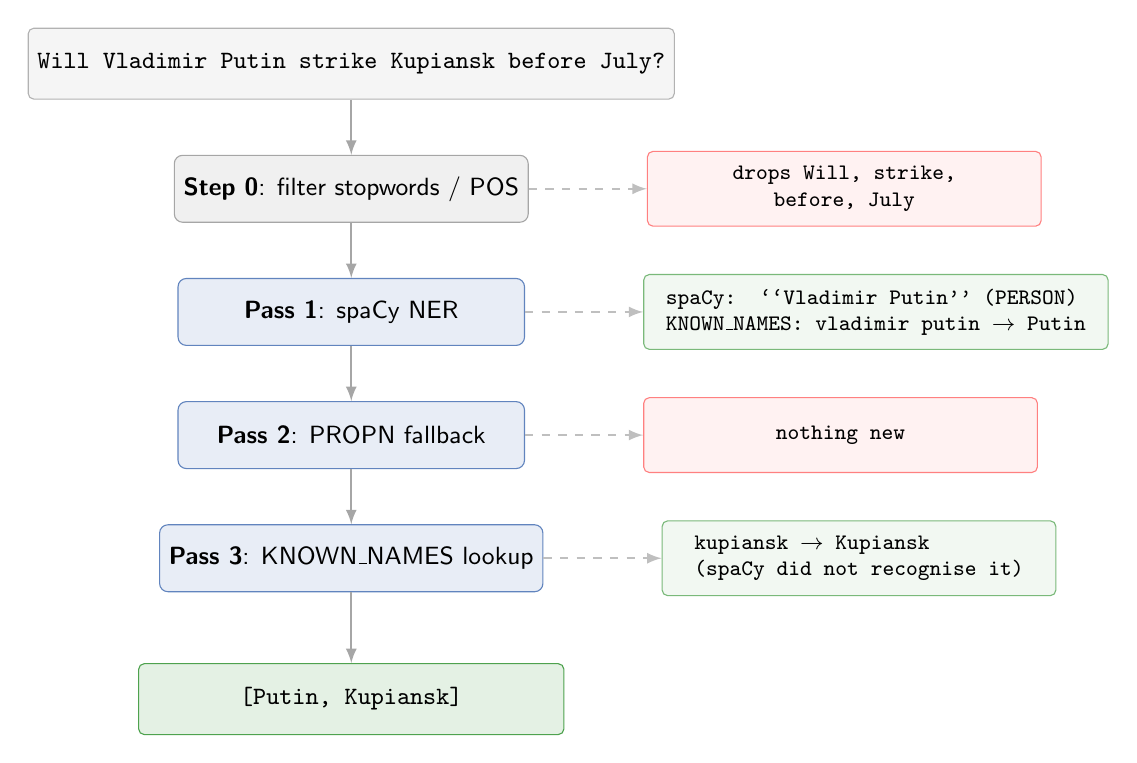
\begin{tikzpicture}[
    qbox/.style   = {rectangle, rounded corners=2pt,
                     draw=gray!60, fill=gray!8,
                     minimum width=6.8cm, minimum height=0.9cm,
                     font=\small\ttfamily, align=center},
    filter/.style = {rectangle, rounded corners=3pt,
                     draw=gray!70, fill=gray!12,
                     minimum width=4.4cm, minimum height=0.85cm,
                     font=\small\sffamily, align=center},
    stage/.style  = {rectangle, rounded corners=3pt,
                     draw=PolyBlue!70, fill=PolyBlue!10,
                     minimum width=4.4cm, minimum height=0.85cm,
                     font=\small\sffamily, align=center},
    drop/.style   = {rectangle, rounded corners=2pt,
                     draw=red!50, fill=red!5,
                     minimum width=5.0cm, minimum height=0.95cm,
                     font=\footnotesize\ttfamily, align=center},
    keep/.style   = {rectangle, rounded corners=2pt,
                     draw=ForestGreen!60, fill=ForestGreen!6,
                     minimum width=5.0cm, minimum height=0.95cm,
                     font=\footnotesize\ttfamily, align=left,
                     inner xsep=8pt},
    result/.style = {rectangle, rounded corners=2pt,
                     draw=ForestGreen!80, fill=ForestGreen!12,
                     minimum width=5.4cm, minimum height=0.9cm,
                     font=\small\ttfamily\bfseries, align=center},
    arr/.style    = {->, >=latex, thick, gray!70},
]

% ─── Input question ──────────────────────────────────────────────────────
\node[qbox] (q)
    {Will Vladimir Putin strike Kupiansk before July?};

% ─── Step 0: stopword / POS filter ───────────────────────────────────────
\node[filter, below=0.7cm of q] (f)
    {\textbf{Step 0}: filter stopwords / POS};
\draw[arr] (q) -- (f);

\node[drop, right=1.5cm of f] (f_drop)
    {drops \texttt{Will}, \texttt{strike},\\
     \texttt{before}, \texttt{July}};
\draw[arr, gray!50, dashed] (f.east) -- (f_drop.west);

% ─── Pass 1: spaCy NER ───────────────────────────────────────────────────
\node[stage, below=0.7cm of f] (p1)
    {\textbf{Pass 1}: spaCy NER};
\draw[arr] (f) -- (p1);

\node[keep, right=1.5cm of p1] (p1_keep)
    {spaCy: ``Vladimir Putin'' (PERSON)\\
     \texttt{KNOWN\_NAMES}: \texttt{vladimir putin} $\rightarrow$ \texttt{Putin}};
\draw[arr, gray!50, dashed] (p1.east) -- (p1_keep.west);

% ─── Pass 2: proper noun fallback ────────────────────────────────────────
\node[stage, below=0.7cm of p1] (p2)
    {\textbf{Pass 2}: PROPN fallback};
\draw[arr] (p1) -- (p2);

\node[drop, right=1.5cm of p2] (p2_drop)
    {nothing new};
\draw[arr, gray!50, dashed] (p2.east) -- (p2_drop.west);

% ─── Pass 3: KNOWN_NAMES phrase lookup ───────────────────────────────────
\node[stage, below=0.7cm of p2] (p3)
    {\textbf{Pass 3}: KNOWN\_NAMES lookup};
\draw[arr] (p2) -- (p3);

\node[keep, right=1.5cm of p3] (p3_keep)
    {\texttt{kupiansk} $\rightarrow$ \texttt{Kupiansk}\\
     (spaCy did not recognise it)};
\draw[arr, gray!50, dashed] (p3.east) -- (p3_keep.west);

% Output
\node[result, below=0.9cm of p3] (out)
    {[Putin, Kupiansk]};1
\draw[arr] (p3) -- (out);

\end{tikzpicture}
\caption{Worked example of the three-pass extractor on the question
         \texttt{"Will Vladimir Putin strike Kupiansk before July?"}.
         Step 0 drops stopwords. Pass 1 captures
         \texttt{"Vladimir Putin"} via spaCy NER, which
         \texttt{KNOWN\_NAMES} then normalises to \texttt{Putin}.
         Pass 2 adds nothing. Pass 3 rescues \texttt{Kupiansk}, a
         Ukrainian frontline town that spaCy does not recognise.}
\label{fig:ner_flow}
\end{figure}


\subsubsection*{Vocabulary}

Two dictionaries in \texttt{pipeline\_config.py} control the output
of all three passes. Tables~\ref{tab:stopwords}
and~\ref{tab:known_names} summarise what each does.

\begin{table}[H]
\centering
\caption{\texttt{STOPWORDS} categories (approx.\ 120 entries total).}
\label{tab:stopwords}
\small
\begin{tabularx}{\textwidth}{l X}
\toprule
\textbf{Category} & \textbf{Examples} \\
\midrule
Market boilerplate & \texttt{yes}, \texttt{no}, \texttt{will},
                     \texttt{resolve}, \texttt{market}, \texttt{date} \\
Calendar tokens    & months, \texttt{q1}–\texttt{q4},
                     \texttt{2023}–\texttt{2026}, \texttt{first},
                     \texttt{second} \\
Generic titles     & \texttt{president}, \texttt{prime},
                     \texttt{minister}, \texttt{secretary},
                     \texttt{chancellor} \\
NER noise          & \texttt{god}, \texttt{clock}, \texttt{trillion},
                     \texttt{emergency}, \texttt{victory} \\
\bottomrule
\end{tabularx}
\end{table}

\begin{table}[H]
\centering
\caption{\texttt{KNOWN\_NAMES} transformation categories
         (approx.\ 250 entries total).}
\label{tab:known_names}
\small
\begin{tabularx}{\textwidth}{l X}
\toprule
\textbf{Transformation} & \textbf{Example mapping} \\
\midrule
Name variants       & \texttt{benjamin netanyahu} $\rightarrow$ \texttt{Netanyahu} \\
Demonyms            & \texttt{israeli}            $\rightarrow$ \texttt{Israel}    \\
Abbreviations       & \texttt{u.s.}               $\rightarrow$ \texttt{USA}       \\
Multi-word phrases  & \texttt{gulf leaders summit} $\rightarrow$ \texttt{Gulf Leaders Summit} \\
Out-of-vocab names  & \texttt{pokrovsk}           $\rightarrow$ \texttt{Pokrovsk}  \\
Possessive stripping & \texttt{Israel's}          $\rightarrow$ \texttt{Israel}   \\
\bottomrule
\end{tabularx}
\end{table}


\subsubsection*{Coverage}

Running \texttt{ner\_keywords.py} across all 1,801 resolved markets
with trades yields 328 unique keywords, averaging 1.93
per market. The top 10 account for most of the coverage
(Table~\ref{tab:top_keywords}), and a lot of  keywords
covers one or two markets each. The overall sentiment and financial
coverage breakdown, including markets that produce no keywords at
all, is reported in Section~\ref{sec:sentiment_coverage}.

\begin{table}[H]
\centering
\caption{Top 10 keywords by market coverage.}
\label{tab:top_keywords}
\small
\begin{tabularx}{0.6\textwidth}{X r}
\toprule
\textbf{Keyword} & \textbf{Markets} \\
\midrule
Israel    & 412 \\
Trump     & 396 \\
Iran      & 223 \\
USA       & 182 \\
Russia    & 167 \\
Zelenskyy & 116 \\
Ukraine   & 105 \\
Yemen     & 100 \\
Putin     &  98 \\
Gaza      &  67 \\
\bottomrule
\end{tabularx}
\end{table}




% ── 3.3 Financial Times — ProQuest Corpus and FinBERT ──────────────────────
\subsection{Financial Times --- ProQuest Corpus and FinBERT}
\label{sec:ft_finbert}

The Financial Times track produces weekly sentiment scores for each
market from FT coverage during the market's lifetime. This section runs in four stages: Corpus acquisition, parsing, FinBERT scoring, and weekly aggregation.



\subsubsection*{Corpus Acquisition}
\label{sec:corpus_acquisition}

ProQuest does not expose a bulk download API at the UCD subscription
tier --- articles must be selected through the web interface and
exported as \texttt{.txt} files. A market-by-market download is
therefore not feasible. Queries were constructed manually, guided by
the NER keyword distribution in Section~\ref{sec:ner_keywords}, with
three targeting decisions per query.

\paragraph{Query scope.} Bare single-keyword queries for common
terms like \texttt{"Russia"} or \texttt{"Iran"} return tens of
thousands of FT articles and cannot be practically exported. These
were narrowed to two-keyword AND combinations (e.g.\
\texttt{"Russia" AND "Ukraine"}). For niche entities like
\texttt{"Houthi"}, \texttt{"Kupiansk"}, or \texttt{"Milei"}, the
article count is already bounded and single-keyword queries were
used directly.

\paragraph{Date window.} Each query was constrained to the lifetime
of the markets it supports, with a 30-day lead added before the
earliest market opens to capture the immediate pre-opening news
cycle (Table~\ref{tab:date_windows}).

\begin{table}[H]
\centering
\caption{Date windows for three representative topics.}
\label{tab:date_windows}
\small
\begin{tabularx}{\textwidth}{l l l X}
\toprule
\textbf{Topic} & \textbf{Window} & \textbf{Articles} & \textbf{Rationale} \\
\midrule
\texttt{russia\_ukraine}    & 2023-01 -- 2025-10 & 5{,}132
    & Continuous market coverage throughout the war. \\
\addlinespace[3pt]
\texttt{saudi\_arabia\_usa} & 2025-04 -- 2025-10 & 1{,}133
    & Markets opened spring 2025 around the Gulf Leaders Summit. \\
\addlinespace[3pt]
\texttt{elon\_musk\_trump}  & 2024-12 -- 2025-10 & 2{,}040
    & Markets tracked a specific feud window. \\
\bottomrule
\end{tabularx}
\end{table}

\paragraph{Batching.} ProQuest exports are capped at 500 articles
per batch. High-volume topics required many batches:
\texttt{russia\_ukraine} in 53, \texttt{china\_taiwan} in 35, while
niche topics like \texttt{houthi} and \texttt{bolsonaro} required
a single batch. Batch counts do not map linearly to article counts
because some batch sizes are 100 others are 500.

\paragraph{} In total, 72 topic corpora were acquired spanning
1 February 2023 to 31 October 2025. \texttt{parse\_proquest.py}
(Section~\ref{sec:parsing}) produced 63{,}874 parsed articles;
\texttt{finbert\_scorer.py} (Section~\ref{sec:finbert_scoring})
scored 51{,}647. The ${\sim}19\%$ gap consists of broad
single-keyword corpora that were parsed early in development but
later superseded by narrower two-keyword AND queries, and so were
not carried through to scoring. Table~\ref{tab:corpus_sizes} shows
the 10 largest scored corpora.

\begin{table}[H]
\centering
\caption{Top 10 ProQuest corpora by scored article count.}
\label{tab:corpus_sizes}
\small
\begin{tabularx}{\textwidth}{X r r l}
\toprule
\textbf{Topic} & \textbf{Batches} & \textbf{Articles} & \textbf{Date range} \\
\midrule
russia\_ukraine   & 53 & 5{,}132 & 2024-08 -- 2025-10 \\
china\_taiwan     & 35 & 3{,}390 & 2023-12 -- 2025-10 \\
moscow\_ukraine   & 32 & 3{,}132 & 2024-02 -- 2025-10 \\
gaza\_israel      & 28 & 2{,}668 & 2024-05 -- 2025-10 \\
hamas\_israel     & 22 & 2{,}140 & 2024-06 -- 2025-10 \\
iran\_usa         &  5 & 2{,}051 & 2023-11 -- 2025-10 \\
elon\_musk\_trump &  5 & 2{,}040 & 2025-01 -- 2025-10 \\
iran\_israel      &  4 & 1{,}757 & 2024-05 -- 2025-10 \\
trump\_putin      & 19 & 1{,}648 & 2024-11 -- 2025-10 \\
netanyahu         &  3 & 1{,}472 & 2024-09 -- 2025-10 \\
\bottomrule
\end{tabularx}
\end{table}



%\inputsection{03_sentiment_pipeline}

%\inputsection{04_exploratory_analysis}

%\inputsection{05_ml_model}

%\inputsection{06_business_case}

% ==========================================================
%  BIBLIOGRAPHY
% ==========================================================
\newpage
\bibliographystyle{plainnat}
\bibliography{bibliography}

% ==========================================================
%  APPENDIX
% ==========================================================
\newpage
\appendix

\section{Data Download}
\label{app:download}

The raw snapshot is retrieved by running the following command from the
project root:

\begin{verbatim}
curl -L -o data/raw/orderFilled_complete.csv.xz \
    https://polydata-archive.s3.us-east-1.amazonaws.com/orderFilled_complete.csv.xz
\end{verbatim}

\noindent This downloads the 5.9\,GB compressed archive directly from
the \texttt{warproxxx/poly\_data} S3 bucket. Full setup instructions
are in the project README at
\href{https://github.com/johnstew324/polymarket-whale-watch}{%
\faGithub\;\texttt{johnstew324/polymarket-whale-watch}}.


\section{Pipeline Source Code}
\label{app:code}

% include key scripts here with \lstinputlisting or verbatim blocks
% e.g. \lstinputlisting[language=Python, caption={filter\_xz.py}]{../src/pipeline/filter_xz.py}

\end{document}